\documentclass[border=10pt]{standalone}
\usepackage{pgfplots}
\pgfplotsset{compat=1.18}
\begin{document}
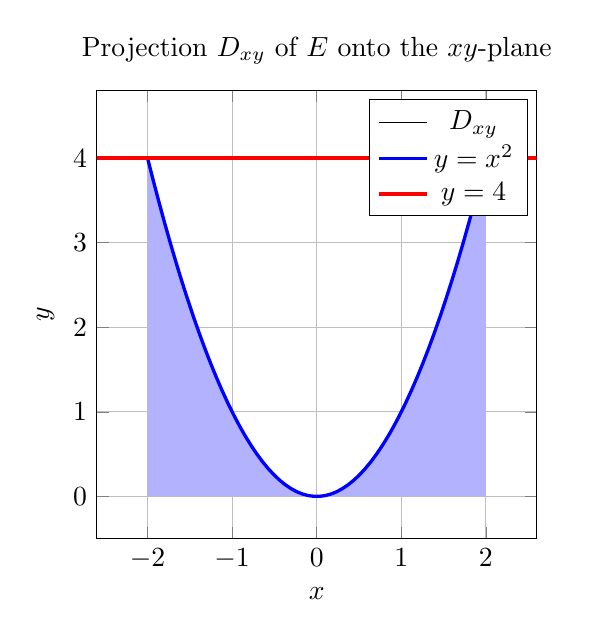
\begin{tikzpicture}
\begin{axis}[
    xlabel={$x$}, ylabel={$y$},
    xmin=-2.6, xmax=2.6, ymin=-0.5, ymax=4.8,
    title={Projection $D_{xy}$ of $E$ onto the $xy$-plane},
    grid, axis equal image]
% shaded region between parabola and y=4
\addplot[fill=blue!30, draw=none, domain=-2:2, samples=60]
    ({x}, {x^2}) \closedcycle;
% parabola
\addplot[blue, very thick, domain=-2:2, samples=60] ({x}, {x^2});
% line y = 4
\addplot[red, very thick, domain=-2.6:2.6] ({x}, {4});
\legend{$D_{xy}$, $y=x^2$, $y=4$}
\end{axis}
\end{tikzpicture}
\end{document}
